\documentclass[a4paper, 11pt, oneside]{book}
\usepackage[a4paper, total={6.5in, 10in}]{geometry}
\usepackage{hyperref}

\usepackage[svgnames]{xcolor}
\usepackage{graphicx}
\usepackage[utf8]{inputenc}
\usepackage[T1]{fontenc}
\usepackage{PTSerif}
\usepackage{listings}
\usepackage{booktabs}
\usepackage{fouriernc}
\usepackage{makecell}
\usepackage{fontawesome}
\usepackage{hyperref}
\usepackage{tabularx}
\usepackage{xspace}
\usepackage{xparse}
\usepackage{amssymb, amsmath}
\usepackage[many]{tcolorbox}
\tcbuselibrary{listings}

\newcommand{\scaresolver}{\href{https://checkmarx.com/resource/documents/en/34965-19196-checkmarx-sca-resolver.html}{\textbf{SCA Resolver}}\xspace}
\newcommand{\cxflow}{\href{https://github.com/checkmarx-ltd/cx-flow}{\textbf{CxFlow}}\xspace}
\newcommand{\cxonecli}{\href{https://checkmarx.com/resource/documents/en/34965-68620-checkmarx-one-cli-tool.html}{\textbf{CxOne CLI}}\xspace}
\newcommand{\cxone}{\href{https://checkmarx.com/resource/documents/en/34965-68517-checkmarx-one-user-guide.html}{\textbf{Checkmarx One}}\xspace}
\newcommand{\cxsca}{\href{https://checkmarx.com/resource/documents/en/34965-18662-checkmarx-sca.html}{\textbf{Checkmarx SCA}}\xspace}
\newcommand{\cxsast}{\href{https://checkmarx.com/resource/documents/en/34965-44074-checkmarx-sast.html}{\textbf{Checkmarx SAST}}\xspace}

\newcommand{\cxtoolkit}{\href{https://github.com/checkmarx-ts/cx-supply-chain-toolkit}{\textbf{Checkmarx Supply Chain Toolkit}}\xspace}
\newcommand{\cxtoolkitpath}[2]{\href{https://github.com/checkmarx-ts/cx-supply-chain-toolkit/#1}{\textbf{Checkmarx Supply Chain Toolkit #2}\xspace}}

\newcommand{\cxflowplusplus}{\href{https://github.com/orgs/checkmarx-ts/packages}{\textbf{CxFlow++}}\xspace}

\newcommand{\cxflowplusplustag}{\texttt{cxflowplusplus:latest}}

\newcommand{\sysbox}{\href{https://github.com/nestybox/sysbox}{\textbf{Sysbox}}\xspace}



\begin{document}

\begin{titlepage}
    \thispagestyle{empty}
    \centering
    
\includegraphics[scale=.4]{graphics/cx_logo-dark.png}
    \vfill
    \textcolor{Sienna}{\Huge Checkmarx Supply Chain Toolkit\\0.0 (Development)}
    \vfill
    {\Large\textbf{Nathan Leach, CSSLP\\Checkmarx Principal Solution Architect}}
\end{titlepage}

\newpage


\chapter*{Quickstart}

If you are not familiar with supply chain scanning and
dependency resolution or want to understand how it works, please
start with the Part \ref{part:background}.


\noindent\\If you are trying to integrate supply chain scanning into
you SDLC, Part \ref{part:operation} covers several related topics:

\begin{itemize}
    \item If you are trying to integrate scanning in an existing CI/CD pipeline by \\
    extension of a container that executes a build stage in your pipeline, \\
    please start with Chapter \ref{chap:ext_build_env}.
    \item If you are trying to automatically select the correct build environment for a \\
    supply chain scan invoked via a web hook, please start with Chapter \ref{chap:build_env_affinity}.
    
\end{itemize}



\tableofcontents

\newtcblisting{xml}[3]{
    listing only,
    title=<#1> #2 #3,
    width=\textwidth,
    listing options={
        basicstyle=\small\ttfamily,
        breaklines=true,
        columns=fullflexible,
    },
}

\newtcblisting{code}[3]{
    listing only,
    title=#1 #2 #3,
    width=\textwidth,
    listing options={
        basicstyle=\small\ttfamily,
        breaklines=true,
        columns=fullflexible,
    },
}


\part{Background}\label{part:background}
\chapter{Scan Integration Challenges}
\section{Understanding Dependency Trees}


Software defines dependencies typically by specifying packages directly
consumed by the software in the build instructions.  These are referred to as
\textit{direct dependencies}.  Each direct dependency may also have
dependencies; dependees of dependencies are referred to as 
\textit{transitive dependencies}.  Each dependency of software can be an
internally developed private package or a publicly available open source package.
\footnote{Commercially developed, closed-source third-party packages are grouped into the
category of open source packages for ease of explanation.}
Figure \ref{fig:dependency_tree} shows an example of a dependency tree.

The dependency tree can have a varying depth depending on the composition
of all dependencies.  If one to review the dependency tree of Hadoop, for
example, a very deep dependency tree with a large variety of packages and
licenses would be observed.  The red boxes in Figure \ref{fig:dependency_tree}
show packages that were detected as having known vulnerabilities.

\begin{figure}[h]
    \caption{Example Dependency Tree}
    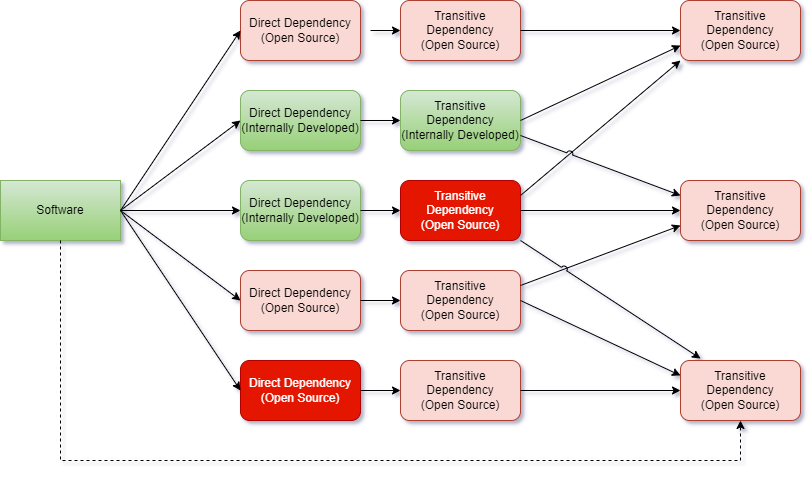
\includegraphics[width=\textwidth]{graphics/dependency_tree.png}
    \label{fig:dependency_tree}
\end{figure}


\subsection{How Detection of Vulnerable Dependencies Can Fail}\label{sec:missing_vulnerable_dependencies}


\subsubsection{Dependency Resolution Happy Path}

One of the potentially vulnerable packages in Figure \ref{fig:dependency_tree} 
is an open source direct dependency of the software.  The detection in this
case is very simple since the dependency is specifically referenced in
the software's build script.  The package is open source, making it well known
and generally available for dependency resolution. Provided the tooling that
can resolve the dependency and a network path to the public repository
is available, the dependency can be resolved.


\subsubsection{Unavailable Private Packages}

The other potentially vulnerable package exhibited in Figure 
\ref{fig:dependency_tree} is a transitive dependency of an internally 
developed direct dependency. A prerequisite of discovering a potentially 
vulnerable package that is a dependee of an internally developed package
is that the internally developed package is available at the time of 
dependency resolution.  

It is often the case that an 
internally developed package is not publicly
available; private packages are typically available through private
package repositories hosted on the organizations internal network.
If that private package repository is not accessible over the network,
the private package and its transitive dependencies will not be available.
The challenges presented in detecting vulnerabilities 
in transitive dependencies of private packages are discussed in detail
in Section \ref{sec:execution_environment}.

\subsubsection{Proper Tooling is Unavailable or Misconfigured}

If the tools required to perform a dependency resolution are not available,
it is apparent that the dependency resolution will fail.  Along with
having the correct tools available, the tools need to be correctly configured.
For example, if a private package repository requires login credentials, 
the dependency resolution will fail unless the tooling configuration provides
those login credentials.

\subsubsection{Improperly Defined Direct Dependencies}

Figure \ref{fig:dependency_tree} depicts a dashed line from the software to a
transitive dependency.  When developers are writing software, it is often
possible to reference packages via namespace.  If a referenced package happens to be
pulled in as a node on the dependency tree below a direct dependency, the
developer may see that a compile and execution works due to the dependency
being resolved as part of the build order.  Since the dependency
is referenced directly in the software, it should be defined as a direct
dependency.  Software can exist and build for years without anyone ever realizing
that the build definition is technically wrong.

This often manifests as a confusing issue where supply chain scans produce one
set of results if performed pre-build when compared to the scan performed post-build.
This is because the build order will cause dependencies to properly resolve by
order of reference.  This downloads and locally caches all required dependencies
and makes them available for the supply chain scan's dependency resolution after the
build.

When performed pre-build, the dependency resolution is usually performed in the order
the build steps are defined rather than in the order of build step dependencies.  This means
that it is possible for some of the dependency resolution to fail
since missing dependencies are not in the local cache.

\subsubsection{Cached Deprecated Dependencies}

When using a non-ephermal build environment that would be commonly known as a "build box," 
modification of these environments are often avoided.  It is not uncommon for build box
to have a software environment that is extremely out of date; no one touches it 
since there is not a reason to fix something that isn't broken.  Eventually no one
knows how the build box is configured to work, no one remembers how it needs to be configured,
and all attempts at creating a new build box cause the build to fail.  Most developers
dread build environment changes.

A side effect of a non-ephermal build environment is that each build execution can mutate
the environment.  Package management tools will typically cache packages downloaded as part
of the dependency resolution.  Unless the build tooling specifically prevents this or the
cache is purposefully cleared periodically, the packages typically stay on the build box
for the entire life of the build box.

Package repositories, however, have no reasonable expectation of keeping all historic packages
available in perpetuity.  It is often the case that both private and public package
repositories will purge deprecated packages.  It is also possible the package maintainers
may decide they no longer want to make the packages available and delete the packages
from the package repository.  Since the build works and no one touches the build box, 
any packages no longer available in a package repository will continue to be available in the
build box package cache.  It may take many years before anyone realizes the package
is no longer publicly available.

When the supply chain scan is executed outside of the environment where the package
cache contains the no-longer-available package, there is no way to resolve the package.
This leads to a failure to generate an accurate dependency tree.

Many organizations have moved to ephermal build environments, such as using containers, 
to avoid these issues.  The ephermal environment has a definition that will produce the
environment to be exactly correct each time it is regenerated.  When an ephermal environment
finishes a build, all mutations of the environment are discarded when the ephermal
environment exits.  If using an ephermal build environment, the build will fail immediately
upon trying to retrieve a package that is no longer available.



\section{Execution Environment}\label{sec:execution_environment}

Performing a software build requires the build activities to execute in the
proper execution environment.  The execution environment is often configured
as a "build box" or a container defined as the execution environment in
a pipeline build stage.  The build environment will typically have all the
tools and configuration required to perform a software build intended 
to yield an package 
containing executable software.  As part of the build, the resolution of 
dependencies is typically part of one or more build steps.  This is often 
required for the software to compile and/or to produce
a distributable build output.\footnote{Not all languages require a compile
or to have dependencies available for the distributable packaging.
The hypothetical scenario discussed is that the dependencies need to be
available at some point during software development if they are 
used by the software at runtime.}

Obtaining an accurate dependency resolution requires the dependency tree to be
resolved in the correct execution environment.  This applies to not only the
availability of the tools and configuration required to resolve 
the dependencies, but also to
the network accessibility where the dependency resolution is executed.  It
frequently the case that dependencies are obtained by network services
accessible only when originating a request from an organization's network. 
In cases such as the one illustrated in Figure \ref{fig:dependency_tree},
the vulnerable transitive dependency of an internally developed package may
not be detected in some scenarios.



\subsubsection{Execution Environment Happy Path}\label{sssec:happy_path}

Figure \ref{fig:dependency_resolution_happy_path} illustrates the concept
of a basic dependency resolution happy path.  In the diagram, the supply chain
scan is added to an existing pipeline to perform dependency resolution
and obtain the dependency tree required for the scan.  The dependency tree is
then sent to the scanning service where the tree is assessed for 
vulnerable packages.

The reason this works is that the dependency resolution is executed inside of
the very same environment used to build the software.  Not only is the correct 
tooling available and properly configured, it is run with the same network
accessibility that allows any private packages to be resolved during the build.

A build environment may serve one or more projects that have the same tooling,
configuration, and network accessibility requirements.  As part of configuring
the ability to build the software, the correct environment for the project
is often defined as part of the pipeline definition.  

As an example, refer to the 
\hyperref[listing:ado_pipeline]{\texttt{Azure Devops Pipeline Example}} listing.
It can be observed in the example pipeline definition that the \texttt{container} 
or \texttt{pool} directives can be used to give the pipeline stage execution an affinity 
for a specific build box or container. When the dependency resolution and supply chain scan
is executed, the execution is in an environment that contains all the tools
needed for a successful scan.



\begin{figure}[h]
    \caption{Dependency Resolution Execution Happy Path}
    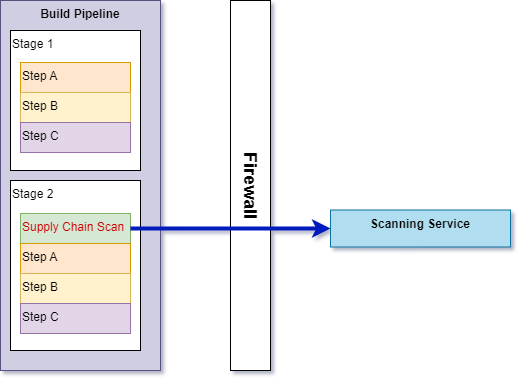
\includegraphics[width=\textwidth]{graphics/dependency_resolution_happy_path.png}
    \label{fig:dependency_resolution_happy_path}
\end{figure}



\label{listing:ado_pipeline}
\begin{code}{Azure Devops Pipeline Example}{}{}
trigger:
    - master

pool:
    vmImage: ubuntu-latest

jobs:
    - job: SCAResolver
        pool:
            vmImage: ubuntu-latest

        container: 
            image: cxnleach/scaresolver-general-build-ado:latest

        steps:
            - script: /sandbox/resolver/ScaResolver -h
\end{code}




\subsubsection{Generic Execution Environment}\label{sssec:generic_environment}

Figure \ref{fig:dependency_resolution_generic_env} depicts a build pipeline that
submits the code or build definition files to a remote service for dependency
resolution and supply chain scanning.  It is very similar to the scenario
described previously in \hyperref[sssec:happy_path]{\textit{Execution Environment Happy Path}}
with the difference being that the dependency resolution is executing in
an execution environment provided by the remote system.  The remote system may not have the
ability to define a specific execution environment for dependency resolution as can
be done within a pipeline definition.

In this scenario, the generic build environment must have properly installed and configured
all tools required to successfully perform a dependency resolution.  In some cases, 
the tooling installation and configuration requirements is simple and this will work.  There
are other cases where this may not be so simple:

\begin{itemize}
    \item The dependency resolution requires older or newer versions of the build tools.
    \item The build tools are not compatible with the remote platform's build environment.
    \item Internally built or third-party licensed tools are required.
    \item Specific tooling configurations are required to perform the build.
\end{itemize}

If the tooling and configuration is not correctly defined in the generic environment,
the dependency resolution may not accurately produce a dependency tree.

\begin{figure}[h]
    \caption{Dependency Resolution Generic Execution Environment}
    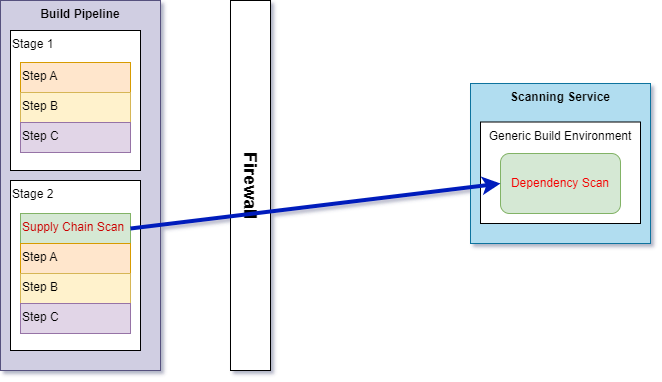
\includegraphics[width=\textwidth]{graphics/dependency_resolution_generic_env.png}
    \label{fig:dependency_resolution_generic_env}
\end{figure}



\subsubsection{Remote Execution Environment}\label{sssec:remote_environment}

A remote execution environment is a variation of the 
\hyperref[sssec:generic_environment]{\texttt{Generic Execution Environment}}.  In this
environment, the build environment can be generic or it can have the correct tooling
and configuration necessary to produce a build.  The challenge here is that the network
paths available to the remote execution environment may not allow for an accurate
dependency tree to be generated.

Figure \ref{fig:dependency_resolution} shows the diagram of the network connections
used during the dependency resolution.  The remote environment will generally have
no issues accessing public package repositories to resolve open source direct and transitive
dependencies.  The red line shows an attempted network connection to a package
repository that may be accessible only from within the corporate network.  When the
supply chain scan submits the scan so that dependency resolution occurs in the
remote environment, the network connection may not be available.  

If \texttt{Step A} of the pipeline's \texttt{Stage 2} is executed after the supply chain
scan, it is performed inside the corporate network.  The green line indicates that it can 
reach the internal package repository.  The internal package repository can be reached
since the execution of \texttt{Step A} is performed on the corporate network.

\begin{figure}[h]
    \caption{Dependency Resolution Remote Execution Environment}
    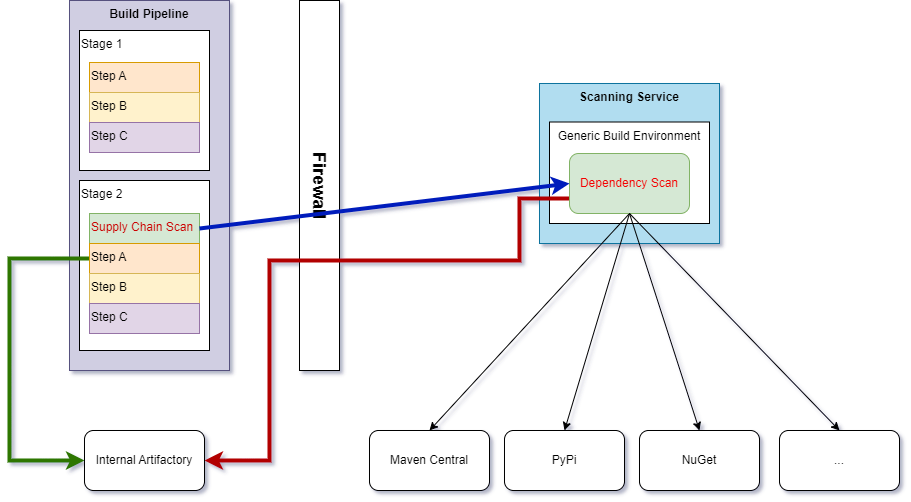
\includegraphics[width=\textwidth]{graphics/dependency_resolution.png}
    \label{fig:dependency_resolution}
\end{figure}







\part{Operation}\label{part:operation}

\section*{Preface}

Many supply chain scan integrations are performed similar to the integration
described in Section \ref{sssec:happy_path}
\hyperref[sssec:happy_path]{\textit{Execution Environment Happy Path}}. It
is then often discovered that only a small number of projects can produce
an accurate dependency tree due to the issues described in Section
\ref{sssec:generic_environment}
\hyperref[sssec:generic_environment]{\textit{Generic Execution Environment}} or
Section \ref{sssec:remote_environment}
\hyperref[sssec:remote_environment]{\textit{Remote Execution Environment}}.

\noindent\\This part of the manual will provide some options for integrating
supply chain scans into workflows executed by tools running
in a customized build environment on the local corporate network.


\chapter{Integrating \scaresolver into Build Environments}\label{chap:ext_build_env}

If you've determined that your dependency resolution scanning does not execute properly
in a \hyperref[sssec:remote_environment]{\textit{Remote Execution Environment}}, \scaresolver
is the solution for executing the dependency resolution in an environment you have defined.
The Checkmarx \scaresolver is the scan command line tool that invokes 
dependency scans locally.  It can be invoked directly or as part of another
tool such as \cxflow, the \cxonecli, or other Checkmarx plugins.

\cxsca is a standalone product that provides a portal that manages supply chain vulnerability scans.  This is
typically used in combination with the \cxsast product to provide both static analysis and supply-chain vulnerability
scans.  \scaresolver can communicate directly with \cxsca to upload data from the locally executed supply-chain
scan, which would have presumably executed in your customized build environment.

\cxone is a product that combines multiple scan types, including supply-chain vulnerability scans, into a single
view.  Scans are typically invoked using the \cxonecli where the type of scan to invoke is defined as part
of the CLI execution parameters.  By default, the \cxonecli will use the 
\hyperref[sssec:remote_environment]{\textit{Remote Execution Environment}} to perform the supply-chain
vulnerability scan.  The \cxonecli can be given a path to the \scaresolver executable to allow
the supply-chain vulnerability scan to execute in your customized build environment.  The \cxonecli the uploads
the results to \cxone for final analysis that reports any potentially vulnerable packages.


\noindent\\This section documents methods for integrating the execution of \scaresolver into your
build environment.


\section{Deploying on a Build Agent}

When builds are executed on a specific build agent (a.k.a. "The Build Box"),
the invocation of \scaresolver will typically be scripted to execute
within a pipeline stage.  In this scenario, the \scaresolver should be
installed on all build agents that will run pipelines that have scripted
a supply chain scan invocation.  This is the most simple scenario and applies
when using \scaresolver with \cxsca or \cxone.

Note that in this scenario, updates to \scaresolver will need to be
periodically installed.  There are likely several tools on the build agent
that need periodic update; \scaresolver will simply be one additional
tool that requires occasional update.

\section{Modifying a Containerized Build Environment}

A variation of the build agent deployment is found when containerized
build environments are defined as the execution environment for
pipeline stages.  The supply chain scan invocation is scripted similar
to how it would be invoked when using a build agent.  The main difference
is that the pipeline stage is configured to execute inside a specified
container image.  The container image contains all the tools required
to successfully build the software, which means that an accurate
dependency tree can also be generated if the \scaresolver is invoked
in that build environment.

In this integration scenario, the container definition can be modified to install \scaresolver
as part of the container build.  The pipeline scripting running in the container
will invoke \scaresolver as it would invoke any other tool in the scripted
build steps.  

\section{Containerized Build Environment Extension}\label{sec:extending_environment}

Often it is difficult to modify the build agent installation or the build
container definition to add \scaresolver.  It may also present some
difficulties in deployment for some pipeline architectures.  Another option
is to create new container instances that derive from already defined build
environments.  This has several advantages:

\begin{itemize}
    \item No instability can be introduced into known-stable build environments.
    \item The \scaresolver updates can be applied without modifying any 
    containerized build environments.
    \item Deployment of updates is a simple rebuild of the extended containers.
    \item The \cxtoolkit provides a way to generate the extended build 
    environment image for build images running on popular Linux distributions.
    \item The image created with the \cxtoolkit also provides some isolation of 
    dependency resolution activities to avoid some attacks associated with 
    malware embedded in typo-squatted packages.
\end{itemize}

\noindent\\The "build-environment" components can be obtained from the \cxtoolkitpath{releases/latest}{Releases}.


\subsection{Creating Extended Images}

The build-environment components contains a \texttt{Dockerfile} is multi-stage where stage names
specify the correct variation of Linux\footnote{There is currently no support for Windows base images.}
in the base image.  The stage names are intended to align 
with popular base images used to create build environments.  The \texttt{Dockerfile} stages
execute the commands specific to the Linux OS distribution of the base image to properly configure
\scaresolver.

Any image that can be pulled from the public Docker Hub or a private docker registry connected via 
\texttt{docker login} can be defined as the base image.  If the wrong or incompatible stage is specified, 
the container build will fail. To see the base image Linux distribution, one possible method would be
to view the \texttt{/etc/os-release} file found in the base image.  This can be done by executing the following
command:

\noindent\\\\\texttt{docker run ----rm -it ----entrypoint=cat <base image tag> /etc/os-release}


\noindent\\As an example, determining the Linux variation for the \texttt{gradle:latest} image can
be performed with the following command:

\noindent\\\\\texttt{docker run --rm -it --entrypoint=cat gradle:latest /etc/os-release}

\noindent\\The output of \texttt{/etc/os-release} reveals that the Linux variation is Ubuntu, which is a derivative
of Debian.\\\\

\begin{code}{Output of "cat /etc/os-release" from gradle:latest}{}{}
PRETTY_NAME="Ubuntu 22.04.3 LTS"
NAME="Ubuntu"
VERSION_ID="22.04"
VERSION="22.04.3 LTS (Jammy Jellyfish)"
VERSION_CODENAME=jammy
ID=ubuntu
ID_LIKE=debian
HOME_URL="https://www.ubuntu.com/"
SUPPORT_URL="https://help.ubuntu.com/"
BUG_REPORT_URL="https://bugs.launchpad.net/ubuntu/"
PRIVACY_POLICY_URL="https://www.ubuntu.com/legal/terms-and-policies/privacy-policy"
UBUNTU_CODENAME=jammy
\end{code}



\subsection{How to Build an Extended Image}

Building the extended image is done via a \texttt{docker build}\footnote{These instructions can likely be adapted to other container build tools.  Docker is used here since it is
the most commonly used container toolkit at the time this manual was written.} command
using the \texttt{Dockerfile} provided in the \cxtoolkit build-environment.
Docker \href{https://docs.docker.com/build/guide/build-args/}{build arguments} control how the extended image build
is performed.  The most important argument is the \hyperref[sec:BASE]{\textbf{BASE}} build argument.  Other build
arguments are available; details of the available arguments can be found in Appendix \ref{chap:build_args}.



\noindent\\Example build commands:

\begin{code}{Extending Gradle 8.0 Alpine with JDK19}{[with Entrypoint]}{}
docker build -t <your tag> --build-arg BASE=gradle:8.0-jdk19-alpine \
    --target=resolver-alpine .
\end{code}

\begin{code}{Extending Gradle 8.0 Alpine with JDK19}{[without Entrypoint]}{}
docker build -t <your tag> --build-arg BASE=gradle:8.0-jdk19-alpine \
    --target=resolver-alpine-bare .
\end{code}

\begin{code}{Extending Node 19 Alpine}{[with Entrypoint]}{}
docker build -t <your tag> --build-arg BASE=node:19-alpine \
    --target=resolver-alpine .
\end{code}

\begin{code}{Extending Node 19 Alpine}{[without Entrypoint]}{}
docker build -t <your tag> --build-arg BASE=node:19-alpine \
    --target=resolver-alpine-bare .
\end{code}
    
\begin{code}{Extending Node 19 Buster (Debian)}{[with Entrypoint]}{}
    docker build -t <your tag> --build-arg BASE=node:19-buster \
        --target=resolver-debian .
\end{code}

\begin{code}{Extending Node 19 Buster (Debian)}{[without Entrypoint]}{}
docker build -t <your tag> --build-arg BASE=node:19-buster \
    --target=resolver-debian-bare .
\end{code}

\subsection{Extended Image Build Customizations}

There are sub-directories in the build-environment toolkit that are used as part of Building
the extended image.  Items can be add or modified in these directories as appropriate.

\subsubsection{CA Certificates}

The \texttt{cacerts} directory contains Amazon AWS Root CA certs that are used as the CA 
certificate for Checkmarx services.  You can add your own PEM encoded CA certificates in this
directory and it will be included as a trusted CA by the image.

If desired, you can remove the AWS CA files as long as there is at least one PEM
encoded certificate left in the directory during image build.

\subsubsection{\scaresolver Configuration YAML}

The \texttt{default-config} folder contains the \texttt{Configuration.yml} file with a default
configuration for \scaresolver.  It is possible to modify the default configuration so that
common parameter values are not needed to be provided for every invocation of \scaresolver.

\subsection{Dockerfile Targets with Entrypoints}\label{ssec:entrypoint_targets}

If you want to invoke \scaresolver in the extended image in the same way it is invoked from the command
line if it were locally installed, use the entrypoint targets.  If you intend to use the
extended images with the \cxtoolkit 
tools for \hyperref[chap:build_env_affinity]{webhook} scan workflows, extended
images with entrypoints are required.  The current targets that build the extended
image with an entry point are:

\begin{itemize}
    \item \texttt{resolver-alpine}
    \item \texttt{resolver-debian}
    \item \texttt{resolver-redhat}
    \item \texttt{resolver-amazon}
\end{itemize}


\subsection{Bare Dockerfile Targets}\label{ssec:bare_targets}

Containers built with bare targets have no entrypoint and run as root.  
Some CI/CD pipelines will need the ability to execute environment
configuraton commands as root before the stage is executed.  Some CI/CD pipelines
will allow the entrypoint to be overridden and will successfully execute the stage
in the container image.  The Azure Devops pipeline, for example, is not compatible
with images that define an entrypoint.  If your CI/CD pipeline needs a container image without 
an entrypoint, these targets will
produce extended images without an entrypoint:

\begin{itemize}
    \item \texttt{resolver-alpine-bare}
    \item \texttt{resolver-debian-bare}
    \item \texttt{resolver-redhat-bare}
    \item \texttt{resolver-amazon-bare}
\end{itemize}


\section{Extended Containers and Execution Sandboxing}

Building extended images with entrypoint targets will "sandbox" \scaresolver execution 
to the extent possible. This is to allow \scaresolver to execute a dependency resolution
while minimizing the risk of detonating malware payloads found in untrusted build scripts or 
package installation scripts. This is not universally a problem with all dependencies, but 
there is always the possibility for malware delivery via open-source packages. 

\noindent\\In terms of sandboxing, the extended images with entrypoints perform the following sandboxing
activities:

\begin{itemize}
    \item The local user executing the scan has limited privileges.
    \item Code for scanning is provided in a read-only volume map.
    This blocks dependencies that execute code-modifying malware from mutating scanned code.
    \item Output volume maps are write-only, preventing the vulnerability reports and logs
    from being exfiltrated as part of exploitable vulnerability intelligence gathering activities.
\end{itemize}

\noindent\\Nothing is foolproof; don't expect that using this container alone hardens your build
environment.  A threat modeling exercise should be undertaken to understand
if there are other infrastructure changes needed to properly control what is executed in your
build environments.

\subsection{Invoking the Sandbox Container CLI Style}\label{ssec:invoking_cli}

The extended container can invoke \scaresolver or \cxonecli in the same way each CLI tool would be
invoked locally.  Since the container is not executing locally, the code artifacts under scan
need to be mapped to paths inside the container.  Table \ref{table:volume_maps} shows the
container paths where it is appropriate to map volumes during container execution.  

While it is possible
to define your own local container paths for mapping, the paths in Table \ref{table:volume_maps}
have been configured with the container's execution user's permissions set to limit the ability to
interact with the paths as appropriate for the path's purpose.  The \texttt{/sandbox/input} path,
for example, is read-only to prevent modification of the code under scan.

Extended containers with no entrypoint (e.g. the "bare" targets) have the same permissions set
as would be used by extended containers with an entrypoint.  The no-entrypoint targets, however, run
as \texttt{root} which makes the permissions irrelevant.  It is possible to execute the CLI tool as
the sandbox user if desired.  Refer to Appendix \ref{chap:build_args} to see how to detect the user id
of the sandbox user.



\begin{table}[h]
    \caption{Container Volume Mapping Paths}\label{table:volume_maps}      
    \begin{tabularx}{\textwidth}{lcl}
        \toprule
        \textbf{Container Directory} & \textbf{Required} & \textbf{Description}\\
        \midrule
        \texttt{/sandbox/scalogs} & N & \makecell[l]{Used to write \scaresolver logs.}\\
        \midrule
        \texttt{/sandbox/input} & Y & \makecell[l]{This is where the input should be mapped\\
        for \scaresolver inputs.}\\
        \midrule
        \texttt{/sandbox/output} & Y & \makecell[l]{This is the directory where \scaresolver\\
        results files will be written.}\\
        \midrule
        \texttt{/sandbox/report} & Y & \makecell[l]{This is the directory where \scaresolver\\
        report will be written.}\\
        \bottomrule
    \end{tabularx}
\end{table}



\subsubsection{Invoking SCA Resolver}

Extended images with entrypoints can be invoked to use \scaresolver the same way
it would be invoked from the command line with a local install.  Any of the 
\scaresolver
\href{https://checkmarx.com/resource/documents/en/34965-132888-checkmarx-sca-resolver-configuration-arguments.html}{command line arguments}
are passed to the container.  A typical execution is shown below:


\begin{code}{Extended Container Typical CLI Invocation}{[SCA Resolver]}{}
docker run --rm -it \
    -v /my-log-path:/sandbox/scalogs \
    -v .:/sandbox/input \
    -v ./sca-results:/sandbox/output \
    my-container-tag \
    --logs-path /sandbox/scalogs \
    --resolver-result-path /sandbox/output \
    --scan-path /sandbox/input \ 
    <other SCAResolver args...>
\end{code}

Note that options passed to \scaresolver that indicate where to place output should be provided 
with paths prefixed with \texttt{/sandbox} corresponding to the local container paths in 
Table \ref{table:volume_maps}.

\subsubsection{Invoking CxOne CLI with SCA Resolver}

Invoking \scaresolver as a CLI with the extended container is performed by default with the entrypoint
of the extended container.  Using \texttt{cxone} as the first parameter to the extended container will
execute the \cxonecli as if it were invoked from the command line with a local install. A typical
execution is shown below:\\


\begin{code}{Extended Container Typical CLI Invocation}{[CxOne CLI with SCA Resolver]}{}
    docker run --rm -it \
        -v /my-log-path:/sandbox/scalogs \
        -v .:/sandbox/input \
        -v ./sca-results:/sandbox/output \
        my-container-tag \
        cxone \
        scan create \
        --output-path /sandbox/output \
        --sca-resolver /sandbox/resolver/ScaResolver \
        -s /sandbox/input \
        <other CxOne CLI args...>
\end{code}

Note that the \texttt{--sca-resolver} parameter is the container local path where the \scaresolver
executable can be found.

\chapter{Executing Supply Chain Scans in a Pipeline}

\section{Supply Chain Scans with \cxone}

This document does not currently cover integration topics for integrating
\scaresolver invoked in a pipeline with \cxone.  This will be covered in 
future releases.

\chapter{Checkmarx SAST CxFlow Web Hook Integration}\label{chap:build_env_affinity}

% # Sandboxed CxFlow

% This is a re-built CxFlow image that follows the release configuration of the official CxFlow image.  The main purpose
% of this image is to allow the execution of SCAResolver in a (mostly) sandboxed, customer-defined environment.

% This is a work in progress.

% To build the repackaged CxFlow image, something similar to the following build command can be executed:

% `docker build -t cxflow-dispatcher:latest .`

% # Docker in Docker

% This image works by invoking Docker inside the Docker container.  This means the deployment options may be somewhat limited given that
% running Docker inside a Docker container has to be done with the correct deployment environment.

% ## CI/CD Pipeline Deployment

% Compatibility scenarios are TBD.  In most build pipeline tools, the containers running each stage can invoke Docker.

% ## Container Orchestrators and Hosting Infrastructure

% Compatibility with services such as AWS ECS is TBD.  These may not be a viable deployment solution due to the
% privileges needed for Docker in Docker execution.

% ## Instance Deployment

% The testing for this was mostly done with deployment on a compute instance.  Deployment pre-requisites are:

% * Linux instance with a kernel >= 5.12
% * [Sysbox](https://github.com/nestybox/sysbox) installed

% Running the container with the `--privileged` flag may be an option to avoid the need for Sysbox and allow it to run on Linux kernels
% with versions prior to 5.12.  This is TBD.

% ### Installing Sysbox

% This installation was performed on an Ubuntu Linux install.  [Sysbox](https://github.com/nestybox/sysbox) provides a [list of
% compatible Linux distributions](https://github.com/nestybox/sysbox/blob/master/docs/distro-compat.md#supported-linux-distros) that may be an
% alternative to using Ubuntu. The [Sysbox](https://github.com/nestybox/sysbox) installation guide does give instructions for
% [installing Shitfs](https://github.com/nestybox/sysbox/blob/master/docs/distro-compat.md#shiftfs-requirement) to support Linux kernel versions
% prior to 5.12.  This is not a tested scenario.

% To install Sysbox on Ubuntu, the following commands are executed:

% ```
% wget https://downloads.nestybox.com/sysbox/releases/v0.5.2/sysbox-ce_0.5.2-0.linux_amd64.deb
% apt install -y jq docker.io ./sysbox-ce_0.5.2-0.linux_amd64.deb
% ```


% Running CxFlow is performed with a command similar to this:

% ```
% docker run --runtime=sysbox-runc -d <the CxFlow image tag>
% ```

% If the `--runtime=sysbox-runc` option is not included and not using the `--privileged` flag, the image will encounter errors when attempting to invoke Docker.

% ### Logging

% CxFlow logs to the console to maintain running compatibility with the official CxFlow image.  Any dispatcher operations are logged in files found on the 
% container in the directory `/var/log/dispatcher`.  The use of logging files for the dispatcher is to avoid the console logs from being corrupted
% by spontaneous log emissions from the dispatcher.

% # CxFlow Image Compatibility

% All the existing Spring Boot facilities for configuring CxFlow via environment variables work with this image.  Using this image
% in place of the official CxFlow image is compatible as long as there is no need to execute SCAResolver.

% If using SCAResolver, there is more configuration needed.  The container will actively attempt to prevent you from configuring the `SCA_PATH_TO_SCA_RESOLVER` option, 
% providing the path on the command line or setting it in the YAML configuration.  SCAResolver has been replaced in this image with an mediation script that invokes SCAResolver
% in an appropriate container image.

% This image can be used for web hook or command line CxFlow execution.

% # Environment Variables: Options for the Image

% This image supports non-CxFlow environment variables that change how it operates at runtime.

% ## `JAVA_OPTS`
% The default value for this environment variable is `-Xms512m -Xmx2048m`.  This variable can be used to pass options to the Java runtime
% prior to executing the CxFlow jar.

% ## `JAVA_PROPS`
% The default value for this environment variable is `-Djava.security.egd=file:/dev/./urandom`.  This is passed to the Java runtime after `JAVA_OPTS` and before the CxFlow
% jar is executed.  

% ## `SPRING_PROPS`
% The default value for this environment variable is `-Dspring.profiles.active=web`.  This is passed to the Java runtime after `JAVA_PROPS` and before the
% CxFlow jar is executed.  CxFlow has embedded profiles that can be used as a basic set of configurations.  Most of them are outdated; the `web` profile
% usually causes fewer configuration issues.  These are not documented in the CxFlow documentation, so it is best to leave this as-is unless
% advised to do otherwise.

% ## `NO_DOCKERD`

% Set the environment variable `NO_DOCKERD` (no value is required) to prevent starting `dockerd` on startup. 
% Attempting to execute SCAResolver without `dockerd` running will result in an error


% ## `CXFLOW_ALT_JAR_URL`

% If the environment variable `CXFLOW_ALT_JAR_URL` contains a URL to a CxFlow jar, that jar will be downloaded and executed instead of
% the CxFlow jar embedded in the container.


% ## `CXFLOW_JAR_SHA256`

% Set this value with a SHA-256 hash that is expected to match the CxFlow jar.  If replacing the CxFlow jar using `CXFLOW_ALT_JAR_URL`,
% validating the correct hash value before execution is highly encouraged.  If the SHA-256 of the CxFlow jar to be executed does not match
% the provided SHA-256, the jar will not be executed.


% ## `CXFLOW_YAML_URL`

% If the environment variable `CXFLOW_YAML_URL` contains a URL to a CxFlow YAML configuration file, it will be downloaded and set
% as the CxFlow configuration.


% ## `DISPATCHER_YAML_URL`

% If the environment variable `DISPATCHER_YAML_URL` contains a URL to a Dispatcher YAML configuration file, it will be downloaded and set
% as the Dispatcher configuration.


% ## `DEBUG`

% If the variable `DEBUG` exists in the environment, debug logging output will be enabled.


% # SCAResolver Dispatcher

% The exact description of the Dispatcher is TBD.  The basic idea is to execute SCAResolver in a mostly sandboxed execution environment.  The execution environment
% could be a customized build environment.

% The execution environment can be defined as:

% * default - The default image, runtime parameters, environment variables, and SCAResolver parameters used if no runtime environment can be determined
% * tag - The image, runtime parameters, environment variables, and SCAResolver parameters used if a project has a matching tag

% Project tags are obtained from a config-as-code file in the root of the repository (not the CxFlow config-as-code file).  Future enhancements may allow this to be resolved from
% project tags found via the SCA API.

% ## Dispatcher Configuration

% Configuration can be represented by both YAML and Environment variables.  The first YAML file found in `$(pwd)/yaml` when the Dispatcher starts is used
% as the configuration file.  The configuration is evaluated in the following order of precedence:

% 1. Environment variables
% 2. YAML configuration

% An example of the complete YAML configuration can be observed below:

% ```yaml

% docker:
%     login:
%         registry-1.docker.io:
%             username: XXXXXXXXX
%             password: XXXXXXXXX
%         ...
%         ghcr.io:
%             username: XXXXXXXXX
%             password: XXXXXXXXX

% resolver:
%     defaults:
%         containerttl: 15m
%         exectimeout: 10m
%         defaulttag: default

%     images:
%         default:
%             container: test:gradle
%             containerttl: 5m
%             exectimeout: 10m
%             execenv:
%                 FOO: BAZ
%             execparams:
%                 - --log-level=Verbose
%         node: 
%             container: test:node-linux
%             execenv:
%                 FOO: BAR
%             envpropagate:
%                 - MY_ENVIRONMENT_VARIABLE1
%                 - MY_ENVIRONMENT_VARIABLE2

% ```


% ### Section: `docker`

% This section is optional.  It is intended to provide defaults for Docker invocations.

% #### `docker.login`

% This section is a list of container repositories where a `docker login` command will be executed on CxFlow startup.  If the images tags
% configured in the `resolver` section are not stored in the default Docker public repository, configure the repositories here.

% Multiple image repositores can be defined using multiple entries under `docker.login`.


% ```yaml

% docker:
%     login:
%         registry-1.docker.io:
%             username: XXXXXXXXX
%             password: XXXXXXXXX
%         ghcr.io:
%             username: XXXXXXXXX
%             password: XXXXXXXXX
%         my-host.com:
%             username: XXXXXXXXX
%             password: XXXXXXXXX
% ```

% Dashes in hostnames can be represented in environment variable names with a double underscore.  Underscores are not valid in DNS hostnames and are therefore not supported.

% The above example of the `docker.login` YAML has the equivalent environment variables:

% ```
% DOCKER_LOGIN_HUB_DOCKER_IO_USERNAME=XXXX
% DOCKER_LOGIN_HUB_DOCKER_IO_PASSWORD=XXXX
% DOCKER_LOGIN_MY__HOST_COM_USERNAME=XXXX
% DOCKER_LOGIN_MY__HOST_COM_PASSWORD=XXXX
% ```


% ### Section: `resolver`

% This section is used to define parameters for SCAResolver invocation.

% #### `resolver.twostage`

% This is optional, defaults to `true`.

% If `true`, an `online` SCAResolver scan will be split into two stages:

% * The first stage is an `offline` scan.  When invoking the offline scan, credentials for the SCA server are stripped from the command.  This executes the dependency
% resolution without leaving credentials exposed to any scripts that execute as part of the dependency resolution.
% * The second stage is an `upload` where the dependency resolution results are uploaded to the SCA server.

% If set to `false`, an `online` scan will be invoked in a single step.


% #### `resolver.defaults`

% This section is optional; it allows for overriding the hard-coded default values if desired.

% The timespan values here can be represented by simple value strings with numeric indicators indicating time units such as `h` for hours, `m` for 
% minutes, and `s` for seconds.  Example:

% `2h15m30s` means 2 hours, 15 minutes, and 30 seconds

% `15m` means 0 hours, 15 minutes, and 0 seconds

% An example of the `resolver.defaults` section can be observed below:

% ```yaml

% resolver:
%     defaults:
%         containerttl: 15m
%         exectimeout: 10m
%         defaulttag: default
%         delete: False

% ```

% `resolver.defaults.containerttl` - If not provided, this defaults to 1 hour.  This is the length of time a container image will be used after the
% initial `docker pull` command is executed to download the image.  This allows updated images to be retrieved without the need to stop CxFlow.

% `resolver.defaults.exectimeout` - If not provided, this defaults to 30 minutes.  This is the amount of time CxFlow will allow the SCAResolver
% image to execute before killing it and assuming failure.

% `resolver.defaults.defaulttag` - If not provided, this defaults to the value of `default`.  This is the tag of the image configured in
% `resolver.images` used if an unknown tag is requested.

% `resolver.defaults.delete` - If not provided, this defaults to the value of `True`.  Setting this to `False` will prevent the container image created
% for the scan from being deleted.

% The above example of the `resolver.defaults` YAML has the equivalent environment variables:

% ```
% RESOLVER_DEFAULTS_CONTAINTERTTL=15m
% RESOLVER_DEFAULTS_EXECTIMEOUT=10m
% RESOLVER_DEFAULTS_DEFAULTTAG=default
% RESOLVER_DEFAULTS_DELETE=False
% ```

% #### `resolver.images`

% This section is where the image parameters are set for a container matching a tag that indicates which container image to
% use when invoking SCAResolver.

% Each dictionary of key/value pairs configured under the `resolver.images` uses the key value as the image tag.  An example of a configuraton
% for images tagged `default` and `node`.  The containers defined would be instances of [the SCAResolver sandbox](../sandbox) image derived
% from an appropriate build environment base image.

% In each of the sections, the `containerttl` and `exectimeout` values are optional.  If not provided, the corresponding values from the 
% `resolver.defaults` section will be used.


% ```yaml

% resolver:
%     images:
%         default:
%             container: test:gradle
%             containerttl: 5m
%             exectimeout: 10m
%             execenv:
%                 FOO: BAZ
%             execparams:
%                 - --log-level=Verbose
%         node: 
%             container: test:node-linux
%             execenv:
%                 FOO: BAR
%             envpropagate:
%                 - MY_ENVIRONMENT_VARIABLE1
%                 - MY_ENVIRONMENT_VARIABLE2

% ```


% `resolver.images.<tag>.container` - Required.  The container image tag name associated with the configuration tag that will be resolved as
% part of the CxFlow scan execution.  

% `resolver.images.<tag>.containerttl` - Optional.  Uses the corresponding value from `resolver.defaults` if not provided.

% `resolver.images.<tag>.exectimeout` - Optional.  Uses the corresponding value from `resolver.defaults` if not provided.

% `resolver.images.<tag>.execenv` - Optional.  A dictionary of key/value pairs that are emitted in the environment when the container image is executed.  Entries
% with key values that match keys defined in `resolver.images.<tag>.envpropagate` will have the value overwritten by the value found in the propagated environment
% value.

% `resolver.images.<tag>.execparams` - Optional.  An array of values passed to SCAResolver at the end of all other parameters needed to control the
% execution of SCAResolver.  The values here are mainly intended to pass configuration values to dependency resolution tools invoked by SCAResolver.  Passing other values
% to SCAResolver may cause operational conflicts.

% `resolver.images.<tag>.envpropagate` - Optional.  An array of names of environment variables in the CxFlow environment that will be propagated as-is to the 
% executing image environment.

% `resolver.images.<tag>.dockerparams` - Optional. An a key/value dictionary that follows the `**kwargs` key/value pairs supported in the [Docker Python API](https://docker-py.readthedocs.io/en/stable/containers.html#docker.models.containers.ContainerCollection.run) `run` method.


% The above example of the `resolver.images` YAML has the equivalent environment variables:

% ```
% RESOLVER_IMAGES_DEFAULT_CONTAINER=test:gradle
% RESOLVER_IMAGES_DEFAULT_CONTAINERTTL=5m
% RESOLVER_IMAGES_DEFAULT_EXECTIMEOUT=10m
% RESOLVER_IMAGES_DEFAULT_EXECENV_FOO=BAZ
% RESOLVER_IMAGES_DEFAULT_EXECPARAMS_1=--log-level=Verbose
% RESOLVER_IMAGES_NODE_CONTAINER=test:node-linux
% RESOLVER_IMAGES_NODE_EXECENV_FOO=BAR
% RESOLVER_IMAGES_NODE_ENVPROPAGATE_1=MY_ENVIRONMENT_VARIABLE1
% RESOLVER_IMAGES_NODE_ENVPROPAGATE_2=MY_ENVIRONMENT_VARIABLE2
% ```

% ## Resolving the Tag for an SCA Scan

% When an SCA scan is invoked, the `default` image tag is used unless a config-as-code file is provided that explicitly
% defines the image tag to use when executing SCAResolver.

% The config-as-code file named `.cxsca` should be placed in the root of the repository.  The contents should be:

% ```json
% {
%     "version" : "1",
%     "tag" : "<image tag>"
% }
% ```




\part{Appendices}
\appendix
\chapter{Release Notes}

\let\sectionold\thesection

\renewcommand\thesection{v}


\section{1.2}

\begin{itemize}
    \item Fix for issue \#39: \textit{Appendix B.4 should document GROUP\textunderscore ID}
    \item Feature \#38: \textit{Integrate SCAResolver dispatcher with CxOne CLI}
\end{itemize}

\section{1.1}

\begin{itemize}
    \item Documentation updates.
    \item Publish a tarball for the CxFlow++ docker image.
\end{itemize}

\section{1.0}

\subsection*{Initial Release}


\let\thesection\sectionold

\chapter{Build Environment Container Build Arguments}\label{chap:build_args}

\newcommand{\buildarg}[3]{
    \section{#3}\label{sec:#1}
    Usage: \texttt{----build-arg #3=#2}\\
    }

\buildarg{BASE}{<base container image:tag>}{BASE}

The build argument \texttt{BASE} is optional and will default to \texttt{alpine:latest} if not 
provided.  The \texttt{BASE} argument should be the tag of a container image that you have 
defined as appropriate for the \texttt{--target} build stage. Your base image should 
contain all required build tooling that would be used in resolving dependencies when run 
against a project that would normally build with that base image.

\buildarg{CONFIGDIR}{<directory relative to the dockerfile>}{CONFIG\textunderscore DIR}

The build argument \texttt{CONFIG\textunderscore DIR} is optional and will default to \texttt{default-config} 
if not provided.  You can create your custom \scaresolver configuration YAML by creating a 
new directory and copying the contents of \texttt{default-config} to initialize the configuration 
artifacts.  You can then modify the configuration artifacts to fit the configuration needed 
by the generated image.


\buildarg{USERID}{<container host invoking user's user id>}{USER\textunderscore ID}

Defaults to "1000", which is generally the ID of the first non-system user created on a clean
Linux system.  Most CI/CD tools will invoke pipeline stages (and thus container images) from
a user account the defined by the pipeline infrastructure.  Since container host directories or files
mapped to a container volume maintain the user/group ownership ID and permission bits when mapped, 
the container's user/group IDs used to set ownership on the \texttt{/sandbox} directory contents
need to match the IDs in the container host.

At build time, a user with the specified ID will be created if it doesn't exist.  If your base 
container already has the user with the specified ID, the user will be used as the user that 
executes \scaresolver. To detect if you need to change this value, you can execute the following 
command in a stage in your pipeline to 
\href{https://www.cyberciti.biz/faq/understanding-etcpasswd-file-format/}{see the user ID}
running the pipeline steps:


\noindent\\\texttt{getent passwd \$(whoami)}






\buildarg{GROUPID}{<container host invoking user's group id>}{GROUP\textunderscore ID}

Defaults to "1000", which is generally the ID of the first non-system group created on a clean
Linux system.  Most CI/CD tools will invoke pipeline stages (and thus container images) from
a user account the defined by the pipeline infrastructure.  Since container host directories or files
mapped to a container volume maintain the user/group ownership ID and permission bits when mapped, 
the container's user/group IDs used to set ownership on the \texttt{/sandbox} directory contents
need to match the IDs in the container host.

At build time, a group with the specified ID will be created if it doesn't exist.  If your base 
container already has the group with the specified ID, the group will be used as the group that 
executes \scaresolver. To detect if you need to change this value, you can execute the following 
command in a stage in your pipeline to 
\href{https://www.cyberciti.biz/faq/understanding-etcpasswd-file-format/}{see the group ID}
of the user running the pipeline steps:


\noindent\\\texttt{getent group \$(groups)}




\chapter{GitHub Action UID/GID Resolution}\label{chap:gh_action_build_args}

The containers build with the \cxtoolkit are designed to allow invocation
so that code under scan is isolated from mutation by any malware that
is included in the build scripts or third-party dependencies.  This is
primarily done by mapping volumes to the running container with permissions
on the original source location set to disallow writes.  The permissions
on the source location propagate to the container with a UID/GID that, if not
matched correctly in the container, may not allow the source to be read for
scanning.

GitHub actions execute on either self-hosted runners or GitHub-hosted runners.
Knowing the correct UID/GID to supply in the build args \texttt{GROUP\_ID}
and \texttt{USER\_ID} (documented in Appendix \ref{chap:build_args}) will
allow invocation of \cxtoolkit containers to work correctly on the type of
runner appropriate for your environment.


\noindent\\The YAML listing below shows a simple dispatch workflow that
can be invoked to determine the runner's UID/GID.  The output of the
workflow is shown in Figure \ref{fig:uidgid} where the UID for
the GitHub-hosted runner is \texttt{1001} and the GID is \texttt{127}.\\

\begin{code}{Example GitHub Action Workflow for Detecting UID/GID}{}{}
name: UID-GID-Check
on:
    workflow_dispatch:
jobs:
    show-uid-and-gid:
    runs-on: ubuntu-latest

    steps:
        
    - name: Action User and UID
        shell: bash
        run: |
        echo User: $(whoami)
        echo UID: $(id -u)
        
    - name: Action Effective Groups
        shell: bash
        run: |
        echo Primary GID: $(id -g)
        echo Primary GID /etc/group entry: $(getent group $(id -g) )
        echo Effective GIDs: $(id -G)  
\end{code}

\begin{figure}[h]
    \caption{Example GitHub Action Workflow Output}
    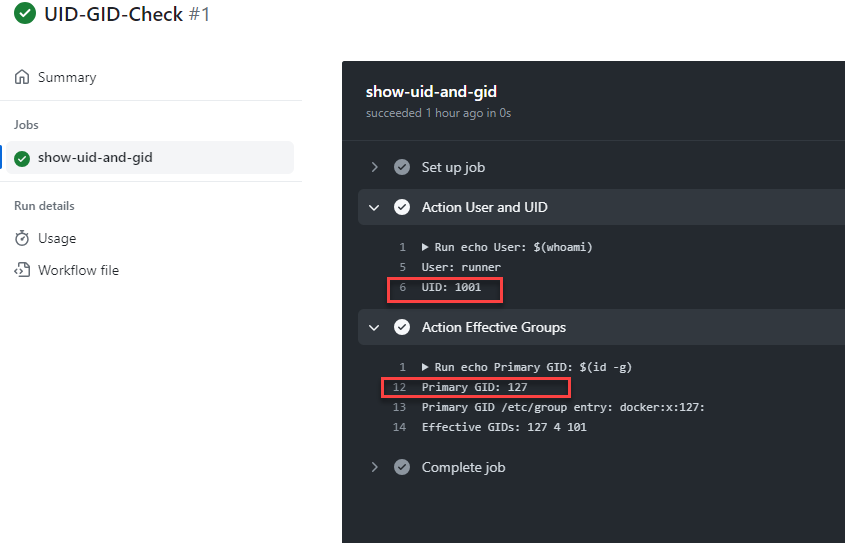
\includegraphics[width=\textwidth]{graphics/uidgid.png}
    \label{fig:uidgid}
\end{figure}

\chapter{\sysbox Installation Instructions}\label{chap:sysbox_install}



This installation was performed on an Ubuntu Linux install.  
The \sysbox GitHub site provides a
\href{https://github.com/nestybox/sysbox/blob/master/docs/distro-compat.md#supported-linux-distros}{list of compatible Linux distributions}
that may be an alternative to using Ubuntu. 

\noindent\\To install Sysbox on Ubuntu, the following commands are executed
\footnote{The \sysbox release available at the time this manual was written may be outdated
at the time of install.  Please verify the latest release artifacts.}:

\begin{code}{Sysbox Installation Steps}{}{}
wget \
https://downloads.nestybox.com/sysbox/releases/v0.5.2/sysbox-ce_0.5.2-0.linux_amd64.deb

apt install -y jq docker.io ./sysbox-ce_0.5.2-0.linux_amd64.deb
\end{code}

\chapter{\cxflowplusplus Image Start Options}\label{chap:image_opts}

\newcommand{\opt}[3]{
    \section{#3}\label{sec:#1}
    Usage: \texttt{----env #3=#2}\\
    }


\opt{JAVAOPTS}{<java runtime options>}{JAVA\_OPTS}

\noindent\\The default value for this environment variable is \texttt{-Xms512m -Xmx2048m}.  This variable can 
be used to pass options to the Java runtime prior to executing the \cxflow jar.

\opt{JAVAPROPS}{<java properties>}{JAVA\_PROPS}

\noindent\\The default value for this environment variable is 
\texttt{-Djava.security.egd=file:/dev/./urandom}.  This is passed to the Java runtime
after \texttt{JAVA\_OPTS} and before the \cxflow jar is executed.  

\opt{SPRINGPROPS}{<spring properties>}{SPRING\_PROPS}

\noindent\\The default value for this environment variable is 
\texttt{-Dspring.profiles.active=web}.  This is passed to the Java runtime after 
\texttt{JAVA\_PROPS} and before the \cxflow jar is executed.  \cxflow has embedded profiles that 
can be used as a basic set of configurations.  Most of them are outdated; the `web` profile
usually causes fewer configuration issues.  These are not documented in the \cxflow documentation, 
so it is best to leave this as-is unless advised to do otherwise.

\opt{NODOCKERD}{1}{NO\_DOCKERD}


\noindent\\Set the environment variable \texttt{NO\_DOCKERD} to prevent starting \texttt{dockerd} 
on startup. Attempting to execute \scaresolver without \texttt{dockerd} running will result 
in an error.


\opt{CXFLOWALTJARURL}{<jar url>}{CXFLOW\_ALT\_JAR\_URL}

\noindent\\If the environment variable \texttt{CXFLOW\_ALT\_JAR\_URL} contains a URL to a \cxflow jar, 
that jar will be downloaded and executed instead of the \cxflow jar embedded in the container.


\opt{CXFLOWJARSHA256}{<sha256 text>}{CXFLOW\_JAR\_SHA256}

\noindent\\Set this value with a SHA-256 hash that is expected to match the \cxflow jar.  
If replacing the \cxflow jar using \texttt{CXFLOW\_ALT\_JAR\_URL},
validating the correct hash value before execution is highly encouraged.  
If the SHA-256 of the \cxflow jar to be executed does not match
the provided SHA-256, the jar will not be executed.

\opt{CXFLOWYAMLURL}{<url>}{CXFLOW\_YAML\_URL}

\noindent\\If the environment variable \texttt{CXFLOW\_YAML\_URL} contains a URL to a \cxflow YAML
configuration file, it will be downloaded and set as the \cxflow configuration.

\opt{DISPATCHERYAMLURL}{<url>}{DISPATCHER\_YAML\_URL}

\noindent\\If the environment variable \texttt{DISPATCHER\_YAML\_URL} contains a URL to a 
Dispatcher YAML configuration file, it will be downloaded and set as the Dispatcher configuration.

\opt{DEBUG}{1}{DEBUG}

\noindent\\If the variable \texttt{DEBUG} is set, debug logging output will be enabled for the
dispatcher.\footnote{Enabling debug logging for \cxflow can be done via the \cxflow configuration.}  




\chapter{Dispatcher Configuration}\label{chap:dispatcher_config}


\noindent\\An example of the complete YAML configuration can be observed below:\\


\begin{code}{Example Dispatcher Configuration YAML}{}{}
docker:
    login:
        registry-1.docker.io:
            username: XXXXXXXXX
            password: XXXXXXXXX
        ...
        ghcr.io:
            username: XXXXXXXXX
            password: XXXXXXXXX

resolver:
    twostage: true
    defaults:
        containerttl: 15m
        exectimeout: 10m
        defaulttag: default

    images:
        default:
            container: test:gradle
            containerttl: 5m
            exectimeout: 10m
            execenv:
                FOO: BAZ
            execparams:
                - --log-level=Verbose
        node: 
            container: test:node-linux
            execenv:
                FOO: BAR
            envpropagate:
                - MY_ENVIRONMENT_VARIABLE1
                - MY_ENVIRONMENT_VARIABLE2

\end{code}


\section{\texttt{docker}}

This section is optional.  It is intended to provide defaults for Docker invocations.

\subsection{\texttt{docker.login}}

This section is a list of container repositories where a \texttt{docker login} command will be 
executed on \cxflowplusplus startup.  If the images tags configured in the \texttt{resolver}
section are not stored in the default Docker public repository, configure the private 
image repositories here.

\noindent\\Multiple image repositories can be defined using multiple entries under 
\texttt{docker.login}.  Each key name under \texttt{docker.login} is the name of the
repository host.  Each repository host key is expecting a \texttt{username} and
\texttt{password} key/value pair.

\noindent\\Example YAML:\\

\begin{code}{\texttt{docker.login}}{YAML Structure}{}
docker:
    login:
        registry-1.docker.io:
            username: XXXXXXXXX
            password: XXXXXXXXX
        ghcr.io:
            username: XXXXXXXXX
            password: XXXXXXXXX
        my-host.com:
            username: XXXXXXXXX
            password: XXXXXXXXX
\end{code}

\subsubsection{\texttt{docker.login} as Environment Variables}

Dots in hostnames are represented in variable names by a single underscore.  Dashes in hostnames can be represented 
in environment variable names with a double underscore.  
Underscores are not valid in DNS hostnames and are therefore not supported.

\noindent\\The above example of the \texttt{docker.login} YAML 
has the equivalent environment variables:\\

\begin{code}{\texttt{docker.login}}{Environment Variables}{}
DOCKER_LOGIN_HUB_DOCKER_IO_USERNAME=XXXX
DOCKER_LOGIN_HUB_DOCKER_IO_PASSWORD=XXXX
DOCKER_LOGIN_MY__HOST_COM_USERNAME=XXXX
DOCKER_LOGIN_MY__HOST_COM_PASSWORD=XXXX
\end{code}

\section{\texttt{resolver}}

This section is used to define parameters for \scaresolver invocation.

\subsection{\texttt{resolver.twostage}}

This is optional; the default is \texttt{true}.

\noindent\\If \texttt{true}, an \texttt{online} \scaresolver scan will be split into two stages:\\

\begin{enumerate}
    \item The first stage is an \texttt{offline} scan.  When invoking the offline scan, 
    credentials for the SCA server are stripped from the command.  This executes the dependency
    resolution without leaving credentials exposed to any scripts that execute as part of the 
    dependency resolution.
    \item The second stage is an \texttt{upload} where the dependency resolution results are
    uploaded to the SCA server.
\end{enumerate}

\noindent\\If set to \texttt{false}, an \texttt{online} scan will be invoked in a single step.

\noindent\\The environment variable \texttt{RESOLVER\_TWOSTAGE} is equivalent to the YAML configuration.


\subsection{\texttt{resolver.defaults}}

This section is optional; it allows for overriding the hard-coded default values if desired.

\noindent\\The timespan values here can be represented by simple value strings with numeric 
indicators indicating time units such as \texttt{h} for hours, \texttt{m} for 
minutes, and \texttt{s} for seconds.  Example:

\noindent\\\texttt{2h15m30s} means 2 hours, 15 minutes, and 30 seconds

\noindent\\\texttt{15m} means 0 hours, 15 minutes, and 0 seconds

\noindent\\An example of the \texttt{resolver.defaults} section can be observed below:\\

\begin{code}{\texttt{resolver.defaults}}{YAML Structure}{}
resolver:
    defaults:
        containerttl: 15m
        exectimeout: 10m
        defaulttag: default
        delete: False
\end{code}


\noindent\\\texttt{resolver.defaults.containerttl} - If not provided, this defaults to 1 hour.  
This is the length
of time a container image will be used after the initial 
\texttt{docker pull} command is executed to download the image.  This allows updated images to be 
retrieved without the need to restart \cxflowplusplus.

\noindent\\\texttt{resolver.defaults.exectimeout} - If not provided, this defaults to 30 minutes.  
This is the amount of time \cxflowplusplus will allow the \scaresolver image to execute before 
killing it and assuming failure.

\noindent\\\texttt{resolver.defaults.defaulttag} - If not provided, this defaults to the value 
of \texttt{default}.  This is the tag of the image configured in \texttt{resolver.images} used if 
an unknown tag is requested.

\noindent\\\texttt{resolver.defaults.delete} - If not provided, this defaults to the value 
of \texttt{true}.  Setting this to \texttt{false} will prevent the container image created
for the scan from being deleted.  The \texttt{false} setting is only recommended for
troubleshooting purposes;
having the \scaresolver containers remain on the \cxflowplusplus runtime container will consume a
significant amount of disk space over time.

\subsubsection{\texttt{resolver.defaults} as Environment Variables}

The above example of the \texttt{resolver.defaults} YAML has the equivalent environment variables:

\begin{code}{\texttt{resolver.defaults}}{Environment Variables}{}
RESOLVER_DEFAULTS_CONTAINTERTTL=15m
RESOLVER_DEFAULTS_EXECTIMEOUT=10m
RESOLVER_DEFAULTS_DEFAULTTAG=default
RESOLVER_DEFAULTS_DELETE=False
\end{code}

\subsection{\texttt{resolver.images}}

This section is where the image parameters are set for a container matching a tag that indicates 
which container image to use when invoking \scaresolver.

Each dictionary of key/value pairs configured under the \texttt{resolver.images} uses the key value 
as the image tag.  The listing below shows an example of a configuration for images 
tagged \texttt{default} and \texttt{node}.  The containers defined would be instances of 
an \scaresolver image derived from an appropriate build environment base image.

In each of the sections, the \texttt{containerttl} and \texttt{exectimeout} values are optional.  
If not provided, the corresponding values from the \texttt{resolver.defaults} section will be used.

\noindent\\\textbf{Note:} Image tags should only contain alphanumeric characters to be compatible with defining
image configurations with environment variables.\\


\begin{code}{\texttt{resolver.images}}{YAML Structure}{}
resolver:
    images:
        default:
            container: my-default-container:latest
            containerttl: 5m
            exectimeout: 10m
            execenv:
                FOO: BAZ
            execparams:
                - --log-level=Verbose
        node: 
            container: my-node-container:latest
            execenv:
                FOO: BAR
            envpropagate:
                - MY_ENVIRONMENT_VARIABLE1
                - MY_ENVIRONMENT_VARIABLE2
\end{code}



\noindent\\\texttt{resolver.images.<tag>.container} - (\textbf{Required}) The container image tag 
name associated with the configuration tag that will be resolved by the dispatcher
during the \cxflowplusplus scan execution.  

\noindent\\\texttt{resolver.images.<tag>.containerttl} - (\textbf{Optional})  Uses the 
corresponding value from \texttt{resolver.defaults} if not provided.

\noindent\\\texttt{resolver.images.<tag>.exectimeout} - (\textbf{Optional})  Uses the corresponding 
value from \texttt{resolver.defaults} if not provided.

\noindent\\\texttt{resolver.images.<tag>.execenv} - (\textbf{Optional}) A dictionary of key/value 
pairs that are emitted in the container's environment when the container image is executed.  
Entries with key values that match keys defined in \texttt{resolver.images.<tag>.envpropagate} 
will have the value overwritten by the value found in the propagated environment value.

\noindent\\\texttt{resolver.images.<tag>.envpropagate} - (\textbf{Optional}) An array of names of 
environment variables in the \cxflowplusplus environment that will be propagated as-is to the 
executing image environment.

\noindent\\\texttt{resolver.images.<tag>.execparams} - (\textbf{Optional}) An array of values passed
to \scaresolver at the end of all other parameters needed to control the
execution of \scaresolver.  The values here are mainly intended to pass configuration
values to dependency resolution tools invoked by \scaresolver.  Passing other values
to \scaresolver may cause operational conflicts.

\noindent\\\texttt{resolver.images.<tag>.dockerparams} - (\textbf{Optional}) A key/value dictionary 
that follows the \texttt{**kwargs} key/value pairs supported in the 
\href{https://docker-py.readthedocs.io/en/stable/containers.html#docker.models.containers.ContainerCollection.run}{Docker Python API} 
\texttt{run} method.

\subsubsection{\texttt{resolver.images} as Environment Variables}

\noindent\\The above example of the `resolver.images` YAML has the equivalent environment variables:\\

\begin{code}{\texttt{resolver.images}}{Environment Variables}{}
RESOLVER_IMAGES_DEFAULT_CONTAINER=my-default-container:latest
RESOLVER_IMAGES_DEFAULT_CONTAINERTTL=5m
RESOLVER_IMAGES_DEFAULT_EXECTIMEOUT=10m
RESOLVER_IMAGES_DEFAULT_EXECENV_FOO=BAZ
RESOLVER_IMAGES_DEFAULT_EXECPARAMS_1=--log-level=Verbose
RESOLVER_IMAGES_NODE_CONTAINER=my-node-container:latest
RESOLVER_IMAGES_NODE_EXECENV_FOO=BAR
RESOLVER_IMAGES_NODE_ENVPROPAGATE_1=MY_ENVIRONMENT_VARIABLE1
RESOLVER_IMAGES_NODE_ENVPROPAGATE_2=MY_ENVIRONMENT_VARIABLE2
\end{code}






\chapter{\cxtoolkit Maintainer's Guide}\label{chap:maintainers_guide}


This section is primarily for the maintainers of the \cxtoolkit.  It is intended
to document any aspects needed to publish a successful release build.


\section{GitHub Action Configuration Pre-Requisites}

Some GitHub action variables and secrets are required to be defined in the repository
for the workflows to work.  Anyone that forks the repository and wants to execute
the workflows will need to define these elements if they wish to test the workflows.

\subsection{Action Variables}

Action variables do not store sensitive information.  Please ensure any additional
variables added never need to store sensitive information.

\subsubsection{Variable: WORKFLOW\_BUILD\_COMPAT}

This is primarily for executing container build unit tests.  These tests will typically
run on a developers desktop without the need for this variable.  The variable adds options
to the \texttt{docker build} command so that it is compatible with the GitHub workflow
execution environment.  It is currently defined as:

\noindent\\\texttt{----load ----build-arg GROUP\_ID=127 ----build-arg USER\_ID=1001}

\noindent\\The UID/GID used by GitHub-hosted runners may periodically change. If 
there are build failures, check that the runner's user has the correct UID/GID.

\subsection{Action Secrets}

The secrets are used in the GitHub action workflows and are used for various functions
that execute inside the workflow.  Some of these values may be required to run some
of the container build unit tests.

\subsubsection{Secret: SCA\_TENANT}
This is a \cxsca tenant name used to perform unit tests.  If this is not provided,
the unit tests that perform scans will be skipped.

\subsubsection{Secret: SCA\_USER}
This is a user in the \cxsca tenant used to perform unit tests.  If this is not provided,
the unit tests that perform scans will be skipped.

\subsubsection{Secret: SCA\_PASSWORD}
This is the password for a user in the \cxsca tenant used to perform unit tests.  
If this is not provided,
the unit tests that perform scans will be skipped.

\subsubsection{Secret: PACKAGE\_USER}
This is the GitHub user that is used for performing workflows that
publish releases and packages.  If this is not provided, the workflow actions
will fail.

\subsubsection{Secret: PACKAGE\_PAT}

This is a PAT associated with the GitHub user defined as the secret
\texttt{PACKAGE\_USER}. If this is not provided, the workflow actions
will fail.

\section{Publishing Releases}

Releases and Pre-Releases are published by workflows found in the GitHub Action
tab on the repository.  The Action tab requires the appropriate permissions
to view; if you're not a member of the maintainer team for \cxtoolkit, you will
not see the action tab.

\subsection{Publish a Release or a Pre-Release}

Publishing a release is as simple as selecting the \texttt{Publish a Release}
workflow in the GitHub Actions tab.  To the right of the screen you will see
a "Run Workflow" button.  When clicked, you will have some options to configure:

\begin{enumerate}
    \item \textbf{Branch} - Select a branch as the source of the release generation.  For
    releases, this should be \texttt{master}.  Pre-releases can be generated from
    any branch as needed.
    \item \textbf{Version tag} - Provide a release version in the form of "x.x".  This value
    will be used to tag the repository and provide version identification information
    for release artifacts.
    \item \textbf{Prelease} - A checkbox that, if checked, will generate a pre-release.
\end{enumerate}

There can be many pre-releases published for a version but only one release of a version.
The workflows will perform code tagging as appropriate for the type of release.  The
workflows will also attempt to validate that the source code is tagged properly before
executing and that tags are removed in the event of a workflow failure.

\subsubsection{Release Publishing Workflows}

A release workflow will fail if a release of the same version has already been
set as a tag in the repo.  While it is possible to work around this by manually
removing repo tags and releases, it is not advised to do so to re-publish a release.
If re-publication of a release is needed, please see Section \ref{sec:republish}


\subsubsection{Pre-Release Publishing Workflows}

Each pre-release will build a tag from the version for which it is a pre-release
and include the build workflow iteration number as part of the tag.  This will allow
for multiple pre-releases to be published for any given release version.

\subsection{Republishing a Release}\label{sec:republish}

Republication of a release is is similar to publishing a release;
all that is required is selecting the \texttt{Republish a Release}
workflow in the GitHub Actions tab.  To the right of the screen you will see
a "Run Workflow" button.  When clicked, you will have some options to configure:

\begin{enumerate}
    \item \textbf{Branch} - Select a branch as the source of the release generation.
    If the re-published release branch and the published release branch differ, things
    may not work so well.
    \item \textbf{Version tag} - Provide a release version in the form of "x.x".  
    This value will be used to fetch the code at the proper tag in the release
    repository.
    \item \textbf{Tag packages as "latest"} - This will set the package tag
    for any published images as \texttt{latest}. 
\end{enumerate}

Republication of a release is limited to full releases only.  The concept of
republishing a release is typically so that newer versions of \cxflow can be
re-packaged into \cxflowplusplus published container images.  Future packaged
components that work similarly will follow this same workflow re-publication
logic.  There are  some things to keep in mind when re-publishing a release:

\begin{itemize}
    \item A release tag must exist for the version being re-published.
    \item The code from the \cxtoolkit is not changed in the release since
    the packaging is performed using code at the release tag.
    \item It will be a good idea to only set the package tag of the latest
    release to \texttt{latest}.  This allows older versions of \cxtoolkit
    to be republished with newer versions of external components incorporated
    in published container images.
    \item While it is possible to set the \texttt{latest} tage on a republished
    image for an older version of the \cxtoolkit, users may have configurations
    that are not backwards compatible.  It is a good idea to avoid re-tagging
    older container images as \texttt{latest}.
\end{itemize}

\section{\cxflowplusplus Container Image Tagging}

The \cxflowplusplus container image is tagged with the \cxtoolkit release or pre-release
tag at the time of the publication.  An additional tag with the \cxtoolkit version
and the incorporated \cxflow version is also provided.  Users of version 1.1,
for example, need only reference the tag \texttt{v1.1} to get the latest version
of \cxflowplusplus.  If \cxflow has a new version released, a republished version 1.1
will retrieve the container image with the latest \cxflow.

It will generally be the case that testing will be performed with \cxflow
versions that are published as future releases.  It is not the intention of the
\cxtoolkit to publish a container image for each past historical version of \cxflow.
As new versions of the \cxtoolkit are released, they will incorporate the latest
version of \cxflow.

If a container image tag for a specific version of \cxflow incorporated into the 
\cxflowplusplus image is not available, please refer to Section \ref{sec:CXFLOWALTJARURL}
for options to retrieve and run a specific \cxflow release at startup.


\end{document}